% !Mode:: "TeX:UTF-8"
% VL 6, gebaut aus part-lernen/09-backpropagation.md (ohne den Induktionsteil,
% der laut kurs-2026-27.md erst in VL 13 als Wiederholung kommt).
% (Dialogmuster und Zeiten: transcripts/vl06-backprop-2025/notiz.md).
% !Mode:: "TeX:UTF-8"
\newcommand{\thepage}{} % to silence a hyperref warning about pdfpagelabels
\RequirePackage[]{silence}
\WarningsOff[hyperref]
\PassOptionsToPackage{log-declarations=false}{xparse}
%\RequirePackage[l2tabu, orthodox]{nag}
\RequirePackage{luatex85} % to make \pdf...= commands work with LuaTeX
\documentclass[aspectratio=169,t]{beamer}
\usepackage{ifthen}
\usepackage[T1]{fontenc}
\usepackage{iftex}
\ifLuaTeX
 \usepackage{fontspec}
 \setmainfont[Ligatures=TeX]{Source Sans Pro}
\else
 \usepackage[utf8]{inputenc}
\fi
\usepackage{german}
\usepackage{newunicodechar}
\newunicodechar{€}{\texteuro}
\newunicodechar{ß}{\ss}
\renewcommand{\SS}{\iffontchar\font"1E9E \symbol{"1E9E}\else SS\fi}
\usepackage{ellipsis}
\usepackage{microtype}
\usepackage{listings}
\usepackage{sourcecodepro}
\lstset{language=Python, basicstyle=\ttfamily}
\usepackage{amsfonts}
\usepackage{amssymb}
\usepackage{amsthm}
\usepackage{fancyhdr}
\usepackage{graphicx}

\newtheorem{proposition}[theorem]{Proposition}

\DeclareMathOperator*{\argmax}{argmax}
\DeclareMathOperator{\supp}{supp}
\newcommand{\E}{\ensuremath{\mathbb{E}}}
\newcommand{\V}{\ensuremath{\mathbb{V}}}

\setbeamercolor{emph}{fg=purple}
\renewcommand<>{\emph}[1]{%
  {\usebeamercolor[fg]{emph}\only#2{\itshape}#1}%
}



\hypersetup{draft=false,colorlinks=false,pdfpagemode=UseOutlines,plainpages=false,
            breaklinks=true,bookmarksnumbered=true,pdfborder=0 0 0,
            pdftitle={Einführung in Deep Learning WiSe 2026/27 HHU},
            pdfauthor={Konrad Voelkel},
            pdfsubject={data science}}

%\documentclass[aspectratio=169,t]{beamer}
\usetheme{hhubeamer} % put the hhu-beamer-theme in /usr/share/texmf/tex/latex/beamer/themes/

% -------------------- Code listings config --------------------
% Define custom colors for syntax highlighting
\definecolor{codegreen}{rgb}{0,0.6,0}
\definecolor{codegray}{rgb}{0.5,0.5,0.5}
\definecolor{codepurple}{rgb}{0.58,0,0.82}
\definecolor{backcolour}{rgb}{0.96,0.96,0.94} % Very light gray/beige
% Configure the listings package
\lstset{
    language=Python,
    backgroundcolor=\color{backcolour},   
    commentstyle=\color{codegreen}\itshape,
    keywordstyle=\color{blue}\bfseries,
    numberstyle=\tiny\color{codegray},
    stringstyle=\color{codepurple},
    basicstyle=\ttfamily\footnotesize, % Use a monospaced font
    breakatwhitespace=false,         
    breaklines=true,      
             % Enable automatic line breaking
    captionpos=b,                      % Caption at the bottom
    keepspaces=true,                 
    numbers=left,                      % Line numbers on the left
    numbersep=10pt,                    % Distance of line numbers from the code
    showspaces=false,                
    showstringspaces=false,            % Don't show weird underscores in strings
    showtabs=false,                  
    tabsize=4,
    frame=single,                      % Add a subtle border around the code
    rulecolor=\color{black!20},        % Border color
  }

\event[]{}
\author[Wintersemester 2026/27]{Dr. Konrad Völkel, Wintersemester 2026/27}

%\title{Data Science, VL 1}
%\date{16.04.2026}


%%% Local Variables:
%%% mode: latex
%%% TeX-master: t
%%% End:


% Fassung mit Dozentennotizen (zweiter Schirm): die nächste Zeile einkommentieren.
% \setbeameroption{show notes on second screen=right}

\graphicspath{{../images/}}

\title[Backpropagation (VL 6)]{Backpropagation\\\large Einführung in Deep Learning, VL 6}
\date{18.11.2026}

\begin{document}

\begin{frame}
  \titlepage

  \note{\textbf{Ablauf, 90 Minuten.} 2025 hat Backpropagation allein 70 Minuten gebraucht,
    deshalb ist diese Sitzung dieses Jahr \emph{nur} Backpropagation --- Aktivierungsfunktionen
    und Autoencoder stehen jetzt in VL 7 und VL 8, wo sie hingehören.\\[2pt]
    \begin{tabular}{@{}rll@{}}
      0--6   & Folien 2--3   & Ziel: den Playground verstehen\\
      6--20  & Folien 4--6   & Setup 1: zwei Neuronen, Update-Regeln von Hand\\
      20--28 & Folien 7--8   & Mehr Dimensionen, mehr Neuronen --- Layer\\
      28--40 & Folien 9--10  & Beispiel 4: Vorwärtsrechnung schichtweise\\
      40--62 & Folien 11--14 & \textbf{Rückwärts differenzieren}\\
      62--72 & Folie 15      & Das Muster: Fehlersignal $\delta_k$\\
      72--80 & Folie 16      & Was PyTorch daraus macht\\
      80--90 & Folien 17--18 & Aufwand, Take-Home, Übungsblatt\\
    \end{tabular}\\[4pt]
    2025 ging es an zwei Stellen zu schnell (Ableitung des Skalarprodukts, Reihenfolge
    beim Transponieren). Beides ist hier eine eigene Folie --- lieber die Beispielsetups
    straffen als hier hetzen.}
\end{frame}

\begin{frame}
  \frametitle{Das Ziel für heute}

  \begin{center}
    \Huge playground.tensorflow.org
  \end{center}

  \bigskip
  \begin{center}
    \normalsize Verstehen können, was da passiert.
  \end{center}

  \note{Wer die Spielaufgabe von letzter Woche gemacht hat, weiß: Die sechs Gewichte für
    XOR von Hand zu setzen, geht --- aber es ist mühsam.
    Genau das Mühsame soll der Gradientenabstieg übernehmen. Dafür brauchen wir den
    Gradienten nach \emph{allen} Gewichten \emph{aller} Schichten. Das ist die Aufgabe
    der Sitzung.}
\end{frame}

\begin{frame}
  \frametitle{Was wir schon haben}

  \begin{center}
    \Large
    $w_{\text{neu}} = w_{\text{alt}} - \rho\,L'(w_{\text{alt}})$\\[16pt]
    \normalsize Was fehlt: $L'$ für ein Netz mit mehreren Schichten.
  \end{center}

  \note{Die Perzeptronregel sagte nichts darüber, wie die vordere Schicht angepasst wird
    (VL 2). Genau diese Lücke schließen wir heute.
    Rahmen, falls jemand fragt, wo das herkommt: differenzierbare Programmierung ---
    alles, was aus differenzierbaren Bausteinen zusammengesetzt ist, lässt sich so
    trainieren.}
\end{frame}

\begin{frame}
  \frametitle{Setup 1: zwei Neuronen}

  \begin{columns}[c]
    \begin{column}{0.5\textwidth}
      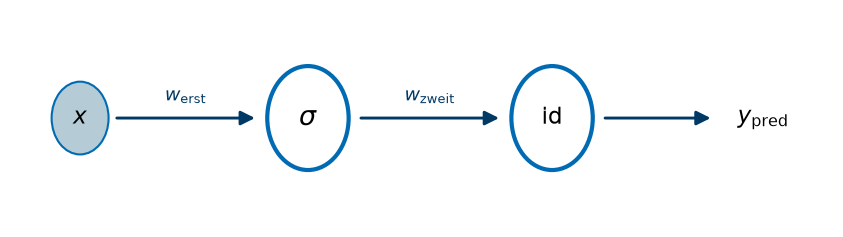
\includegraphics[width=\textwidth]{vl06-two-neurons.png}
    \end{column}
    \begin{column}{0.46\textwidth}
      \Large
      $y_{\text{pred}} = \langle w_2, \sigma(\langle w_1, x\rangle)\rangle$
    \end{column}
  \end{columns}

  \note{Eindimensionale Eingabe, ein Neuron mit $\sigma$, dahinter eines mit der Identität.
    Regression, also MSE-Loss.
    Die Frage ist nur: Was ist $\partial y_{\text{pred}} / \partial W$?
    2025 kam hier die Frage, ob am Ausgang nicht ein Sigmoid fehlt. Gute Gelegenheit für
    die Diskussion: Die Architektur am Ausgang richtet sich nach dem \emph{Wertebereich}
    der Zielfunktion --- bei Regression will man keinen Squeeze auf $(0,1)$.}
\end{frame}

\begin{frame}
  \frametitle{Zwei Bausteine}

  \begin{center}
    \Large
    $\dfrac{d}{dw}\,\sigma(f(w)) = \sigma'(f(w))\,f'(w)$\\[16pt]
    $\dfrac{d}{dw}\,\langle w, x\rangle = x$, \qquad
    $\dfrac{d}{dw}\,\langle v, f(w)\rangle = \langle v, f'(w)\rangle$
  \end{center}

  \note{\textbf{Hier nicht hetzen} --- 2025 kam die Skalarproduktableitung zu kurz, der
    Dozent hat es selbst eingeräumt und empfohlen, sie in $\mathbb{R}^3$ selbst
    nachzurechnen. Das kann man hier auch gemeinsam tun.
    Die Kettenregel oben aus dem Hörsaal abfragen, nicht vorsagen.}
\end{frame}

\begin{frame}
  \frametitle{Die beiden Update-Regeln}

  \begin{center}
    \Large
    $\dfrac{\partial y_{\text{pred}}}{\partial w_2} = \sigma(\langle w_1, x\rangle)$\\[18pt]
    $\dfrac{\partial y_{\text{pred}}}{\partial w_1}
      = \bigl\langle w_2,\, \sigma'(\langle w_1, x\rangle)\,x \bigr\rangle$
  \end{center}

  \bigskip
  \begin{center}
    \normalsize Funktioniert --- aber unübersichtlich.
  \end{center}

  \note{In die Gradientenabstiegsregel eingesetzt, stehen da zwei lange Formeln. Die muss
    man nicht auswendig können; wichtig ist die Beobachtung:
    \emph{Teilausdrücke kommen mehrfach vor} --- das Residuum $y_i - y_{\text{pred},i}$ und
    die Aktivierung der ersten Schicht. Das ist der Keim der ganzen Idee: einmal rechnen,
    mehrfach benutzen.}
\end{frame}

\begin{frame}
  \frametitle{Mehr Dimensionen, mehr Neuronen}

  \begin{center}
    \Large
    Setup 2: $x \in \mathbb{R}^2$ --- die Skalarprodukte werden länger.\\[14pt]
    Setup 3: mehrere Neuronen pro Schicht --- aus $w$ wird $W$.
  \end{center}

  \note{An den Formeln ändert sich strukturell nichts. Das ist die beruhigende Nachricht,
    und sie rechtfertigt, gleich zur Matrixschreibweise zu wechseln.
    2025 kam hier die Frage nach der Dimension des Gewichts „in einem Kreis“ --- die
    Notation ein Kreis je Dimension einmal ausdrücklich klären.}
\end{frame}

\begin{frame}
  \frametitle{Eine Schicht}

  \begin{center}
    \Huge $z_{k+1} = \sigma(b_k + W_k z_k)$
  \end{center}

  \note{Ab jetzt in Matrixschreibweise. Grundphilosophie, die man einmal sagen sollte:
    \emph{Alles ist elementweise, was nicht ausdrücklich anders dasteht} --- $\sigma$ wirkt
    komponentenweise, $W_k z_k$ ist das Matrixprodukt.
    Die Eingabeschicht ist dabei nur ein Name für $z_1 = x$; dort passiert nichts.}
\end{frame}

\begin{frame}
  \frametitle{Beispiel 4: drei Schichten}

  \begin{center}
    \Large
    $f(x) = b_3 + W_3 \tanh\bigl(b_2 + W_2 \tanh(b_1 + W_1 x)\bigr)$
  \end{center}

  \note{Dieses Beispiel begleitet uns durch den Rest der Sitzung --- und ein Rechenbeispiel
    dieser Bauart kommt auf den Übungszettel \emph{und} kann in der Klausur drankommen
    (Aufgabentyp 4). Das ausdrücklich sagen.}
\end{frame}

\begin{frame}
  \frametitle{Vorwärtsrechnung, schichtweise}

  \begin{center}
    \Large
    \begin{tabular}{@{}ll@{}}
      $z_1 = x$ & input\\[4pt]
      $z_2 = \tanh(b_1 + W_1 z_1)$ & 2nd layer\\[4pt]
      $z_3 = \tanh(b_2 + W_2 z_2)$ & 3rd layer\\[4pt]
      $y_{\text{pred}} = b_3 + W_3 z_3$ & output\\[4pt]
      $r = y_{\text{pred}} - y$ & residual\\[4pt]
      $E = \tfrac12 r^T r$ & squared error\\
    \end{tabular}
  \end{center}

  \note{Das ist der \emph{Berechnungsgraph}: nicht die Formel, sondern die Festlegung der
    Rechenreihenfolge --- der Unterschied ist wichtig und kommt in VL 12 wieder.
    Der Faktor $\frac12$ ist reine Bequemlichkeit, er kürzt sich gleich gegen die 2 aus
    der Ableitung des Quadrats.
    Jede Zeile speichert ein Zwischenergebnis. Das brauchen wir gleich alles noch.}
\end{frame}

\begin{frame}
  \frametitle{Rückwärts: die Ausgabeschicht}

  \begin{center}
    \Large
    $dE = r^T\,dy_{\text{pred}}$\\[16pt]
    $\nabla_{b_3} E = r$, \qquad $\nabla_{W_3} E = r\,z_3^T$
  \end{center}

  \note{$y$ ist konstant, deshalb $dr = dy_{\text{pred}}$.
    Die Notation $d$ als Platzhalter erklären: die lineare Änderung bei infinitesimaler
    Änderung der Parameter.
    \textbf{Die Reihenfolge beim Transponieren} ist die Stelle, an der 2025 eine Frage kam
    und vertagt wurde. Kurzfassung: $\nabla_{W_3}E$ ist ein \emph{äußeres Produkt} ---
    Fehler mal Eingabe der Schicht. Wer es genau will: Spur-Trick, steht als Vertiefung
    im Skript; oder komponentenweise
    $\partial E/\partial (W_3)_{jk} = r_j (z_3)_k$, dasselbe Ergebnis.}
\end{frame}

\begin{frame}
  \frametitle{Bekannt vom einzelnen Neuron}

  \begin{center}
    \Large
    Gradient nach der Gewichtsmatrix\\[10pt]
    $=$ Fehler $\times$ Eingabe der Schicht
  \end{center}

  \bigskip
  \begin{center}
    \normalsize Beim einzelnen Neuron war es $(p - y)\,x$ (VL 5).
  \end{center}

  \note{Diese Wiedererkennung ist wichtig: Es ist kein neues Prinzip, nur dieselbe Formel
    pro Schicht.}
\end{frame}

\begin{frame}
  \frametitle{Eine Schicht weiter zurück}

  \begin{center}
    \Large
    $dz_3 = (1 - z_3^2) \odot (db_2 + dW_2 z_2 + W_2\,dz_2)$
  \end{center}

  \bigskip
  \begin{center}
    \normalsize $\odot$ ist elementweise; $\tanh' = 1 - \tanh^2$.
  \end{center}

  \note{Jetzt sind $b_3$ und $W_3$ Konstanten. Die Ableitung von $\tanh$ lässt sich aus
    dem gespeicherten $z_3$ berechnen --- genau wie bei $\sigma' = \sigma(1-\sigma)$ in
    VL 4. Deshalb lohnt es sich, die Zwischenergebnisse zu speichern.
    Wer mag, kann hier das \emph{Recyceln} betonen: $\sigma(Ax)$ und $Ax$ werden beide
    weiterverwendet.}
\end{frame}

\begin{frame}
  \frametitle{Das Muster}

  \begin{center}
    \Large
    $\delta_3 = r$\\[10pt]
    $\delta_2 = (1 - z_3^2) \odot W_3^T \delta_3$\\[10pt]
    $\delta_1 = (1 - z_2^2) \odot W_2^T \delta_2$\\[14pt]
    $\nabla_{W_k} E = \delta_k\,z_k^T$
  \end{center}

  \note{\textbf{Das ist die Folie, die hängen bleiben soll.} Das Fehlersignal wird
    rückwärts propagiert: mit der \emph{transponierten} Gewichtsmatrix multipliziert und
    mit der Ableitung der Aktivierungsfunktion gewichtet.
    Man kann den Graphen an jeder Stelle durchschneiden --- was davor liegt, interessiert
    den Rückwärtsschritt nicht.
    Beobachtung, die 2025 gut ankam: Rückwärts trifft man zuerst das \emph{letzte} Gewicht.}
\end{frame}

\begin{frame}
  \frametitle{Was PyTorch daraus macht}

  \begin{center}
    \Large
    \texttt{loss.backward()} \quad füllt \texttt{.grad}\\[12pt]
    \texttt{optimizer.step()} \quad macht $W \leftarrow W - \rho \nabla_W E$
  \end{center}

  \note{Beim Vorwärtsrechnen merkt sich jeder Tensor mit \texttt{requires\_grad}, aus
    welcher Operation er entstanden ist --- der Berechnungsgraph. \texttt{backward} läuft
    ihn rückwärts ab.
    Das ist genau die Trainingsschleife aus VL 4, jetzt versteht man, was die beiden
    Zeilen tun. Die Details (Graph, Zyklen, gelogene Ableitungen) kommen in VL 12.}
\end{frame}

\begin{frame}
  \frametitle{Was das kostet}

  \begin{center}
    \Large
    ein Vorwärtsdurchlauf\\[8pt] ein Rückwärtsdurchlauf\\[14pt]
    \normalsize $\approx$ das Doppelte einer Inferenz ---\\
    unabhängig von der Zahl der Parameter.
  \end{center}

  \note{Das ist der Grund, warum Deep Learning überhaupt praktikabel ist. Naiv, mit
    finiten Differenzen, bräuchte man eine Auswertung \emph{pro Parameter} --- bei
    Milliarden Parametern undenkbar.
    Take-Home: Backpropagation ist keine neue Mathematik, sondern Kettenregel plus
    Buchführung. In diese Rechnung fließt null Kreativität --- das kann der Computer,
    sobald man ihm für jede Operation die Ableitung nennt.}
\end{frame}

\begin{frame}
  \frametitle{Zur Übung}

  \begin{itemize}\setlength{\itemsep}{8pt}
  \item Ein Rechenbeispiel wie Beispiel 4 --- von Hand, auf einem Übungsblatt
  \item Klausurrelevant (Aufgabentyp 4)
  \item Bitte ohne generative KI
  \end{itemize}

  \bigskip
  \begin{center}
    Nächste Woche: Aktivierungsfunktionen --- und Netze von Hand bauen.
  \end{center}

  \note{Die Rechnung einmal selbst gemacht zu haben, ist der Unterschied zwischen
    „verstanden“ und „zugehört“. In der Klausur kommt sie mit kleinen Zahlen.
    Wer noch Zeit hat: XOR im Playground von Hand lösen bleibt offen --- nächste Woche
    machen wir genau das systematisch.}
\end{frame}

\end{document}

%%% Local Variables:
%%% mode: latex
%%% TeX-master: t
%%% End:
